\documentclass[a4paper,10pt]{article}
\usepackage[utf8]{inputenc}
\usepackage{graphicx}

%opening
\title{Artificial Intelligence \\ notes}
\author{Klara Malinowska}

\begin{document}

\maketitle
\section{Welcome to AI}
\subsection{Terminology}

\paragraph{Fully/partially observable}
The environment is fully observable if what the agent can sense at any point of time is sufficient to make and optimal decision. In partially observable environment the memory of previous states is required to make an optimal decision.

\paragraph{Deterministic/stochastic}
In deterministic environment the effect of an agent actions uniquely determines the outcome. In stochastic environment - the outcome of the action have a certain level of randomness.

\paragraph{Discrete/continuous}
In discrete environment the finally actions choices and things to sense. In continuous environment there is may be unlimited amount of possible actions or things to sense.

\paragraph{Benign/adversarial}
The benign environment does not have an objective that contradicts your objective. In adversarial the environment actively observes the agent actions and counteracts with what it is trying to achieve.

\section{Problem Solving}

Complexity may come from large number of possible choices or from partial observability.

\paragraph{Definition of an problem}
The problem may be defined by a set of states and functions
\begin{enumerate}
  \item Initial state $s$
  \item Action($s$) $\rightarrow$ $a$ There may be a lot of them forming a set ${a_1, a_2, ...}$ and they may be dependent or independent on a current state
  \item Result($s,a$) $\rightarrow$ $s'$ Taking initial state and a chosen action gives us the resulting state.
  \item GoalTest($s$) $\rightarrow$ $s'$ T|F Takes a current states and checks if it is a solution. Returns boolean value.
  \item PathCost($s,a,s,a,s,...$) $\rightarrow$ $n$ Takes sequence of steps and actions and gives a cost of it as a number. Usually is an additive fuction of StepCosts
  \item StepCost($s,a,s'$) $rightarrow$ $n$ Gives a cost of one action as a number.
\end{enumerate}

States space divides into explored part, frontier (which are the farthest state explored) and unexplored part.

A problem solving technology works only if the domain is:
\begin{enumerate}
 \item fully observable (we know exactly the current state)
 \item known (known set of available actions)
 \item discrete(limited amount of possible actions)
 \item deterministic (result of an action is known)
 \item static (nothing changes the space state but we)
\end{enumerate}

\subsection{Path searching}

\paragraph{Tree search vs. graph search} 

The two search algorithms differ in ``having memory'' - remembering which states are already explored. The tree algorithm does not do that, so it can go back with the explored path to the state it has already been in. The graph search remembers where it has already been and thus never goes back to the previously visited states.
\paragraph{Tree search}
\begin{verbatim}
function Tree.Search(problem)
  frontier = {[initial]}
  loop:
    if frontier is empty: return FAIL
    path = remove_choice(frontier)
    s = path.end
    if s is a goal: return path
    for a in actions:
      add [path + a -> Result(s,a)] to frontier
\end{verbatim}

\paragraph{Graph search}
\begin{verbatim}
function Tree.Search(problem)
  frontier = {[initial]}
  explored = {}
  loop:
    if frontier is empty: return FAIL
    path = remove_choice(frontier)
    s = path.end
    add s to explored
    if s is a goal: return path
    for a in actions:
      add [path + a -> Result(s,a)] to frontier 
      unless Result(s,a) in frontier + explored
\end{verbatim}

\paragraph{Breadth first search}
Always chooses the shortest (in term of steps) path to explore next. If there are paths of the same length, it chooses randomly. Is guaranteed to find the shortest (in terms of number of steps) path. Requires storage space of $2^n$ paths to store all the nodes in the frontier.

\paragraph{Uniform-cost search - cheapest first}
It chooses which path to explore next basing on the path cost. Is guaranteed to find the cheapest path, because even if it has already added the goal to the frontier, it firstly explores all the shorter paths and only when the one leading to the goal is the shortest it performs the goal check. Number of paths in the frontier is similar that in the breadth first algorithm.

\paragraph{Depth first search}
It chooses the longest path to explore first. It is not optimal - does not guarantee to find the best solution (path that reaches the goal in the minimal amount of steps). Requires storage space of $n$ to store all the nodes in the frontier.

\paragraph{Number of nodes in the frontier}
It is $2^n$ for the breadth first search and similar in the uniform-cost search. It is $n$ in the depth first search. Thus depth first search requires much less memory than the other two when we save the frontier only. However, if we save also explored space, all three algorithms need the similar amount of memory.

\paragraph{Completeness}
Algorithm is complete if it will always find the optimal path. Breadth first and uniform-cost search algorithms are complete. The depth first search algorithm is not.

\paragraph{Greedy best-first search}
It needs additional information to work, eg. estimate of the distance of the start state to the goal such as straight line distance from the state to the goal. It explores much smaller part of the states space that the uniform-cost search, and therefore shall be faster. However, it may not find the shortest path (if it requires going in the direction ``from'' the goal in some steps) - it is not complete.

\subsection{A* search}
The A* search combines the uniform-cost search and greedy best-first search in its way to determine which path to explore. It chooses the path to explore minimizing on the function h(path) which adds the path cost up to certain state as well as distance from the goal.
\begin{verbatim}
f(path) = g(path) + h(path)
g(path) = path.cost
h(path) = h(s) = current distance to the goal
\end{verbatim}

The A* algorithm will always find the lowest cost path if h(s) function is smaller than a true cost to get to the goal from a current state. It should never overestimate the cost to get to the goal, an thus is an  optimistic. Such an h is called \textbf{admissable} (it is admissible to use it to find a lowest cost path). 

\section{Probability in AI}

\subsection{Probability properties}
\begin{itemize}
\item \textbf{Complementary events} The event $A$ and its complement $\neg A$ are mutually exclusive and exhaustive.
\[p(A) = 1 \Rightarrow p(\neg A) = 1-p \]
\item \textbf{Independence of events} Two events are independent ($A\perp B$) means that the occurrence of one event makes it neither more nor less probable that the other occurs.
\[ A\perp B \Leftrightarrow P(A,B) = P(A)P(B) \]
\item \textbf{Conditional probability} is the probability that event A occurs when the sample space is limited to event B. This is read "the probability of A, given B" and denoted as $P(A\mid B)$.
\[P(\neg A\mid B) = 1-P(A \mid B) \]
\item \textbf{The law of total probability}
If $A_i$ is a set of pairwise disjoint events whose union is the entire sample space, then
\[P(B) = \sum_{i} P(A \mid B_i)P(A_i) \]
\item \textbf{Bayes rule}
\[ P(A|B) = \frac{P(B|A)P(A)}{P(B)} \]
\[ P(A|B,C) = \frac{P(B|A,C)P(A)}{P(B|C)} \]
In this expression $P(A|B)$ is called \textbf{posterior} $P(B|A)$ is called \textbf{likelihood}, $P(A)$ is called \textbf{prior} and $P(B)$ is called \textbf{marginal likelihood}. 

The Bayes rule can be written differently using the law of total probability:
\[ P(A_j|B) = \frac{P(B|A_j)P(A_j)}{\sum_{i} P(A \mid B_i)P(A_i)} \]
It can be also written omitting the usage of $P(B)$ by introducing \textbf{normalizer} $\eta$ defined as
\[ \eta =(P'(A|B)+P'(\neg A|B)) \]
where
\[ P'(A|B) = P(B|A)P(A) \]
\[ P'(\neg A|B) = P(B|\neg A)P(\neg A)\]
Than the Bayes rule can be written as
\[ P(A|B) = \eta P'(A|B) \]

\item \textbf{Conditional independence} The probability of outcome of two events $T_1$ and $T_2$ is dependent of the state of the event C. Those two events are conditionally independent independent given C if
\[ P(T_2|C,T_1)=P(T_2|C) \]
That means that if we know the outcome of event $C$, the probability of outcomes of event $T_2$ does not depend of the outcome of the event $T_1$. The conditional independence of events $T_1$ and $T_2$ given the outcome of event C is denoted as:
\[T_1 \bot T_2 | C \]
\item Conditional independence does not imply the absolute independence, and absolute independence does not imply conditional independence.

\end{itemize}

\subsection{Bayes network}

A Bayes network is a probabilistic graphical model that represents a set of random variables and their conditional dependencies via a directed acyclic graph. The nodes of the graph represent the variables, and the edges represent the conditional dependences. 

\subsubsection{Basic types of Bayes networks}

\begin{figure}[h!]
\centering
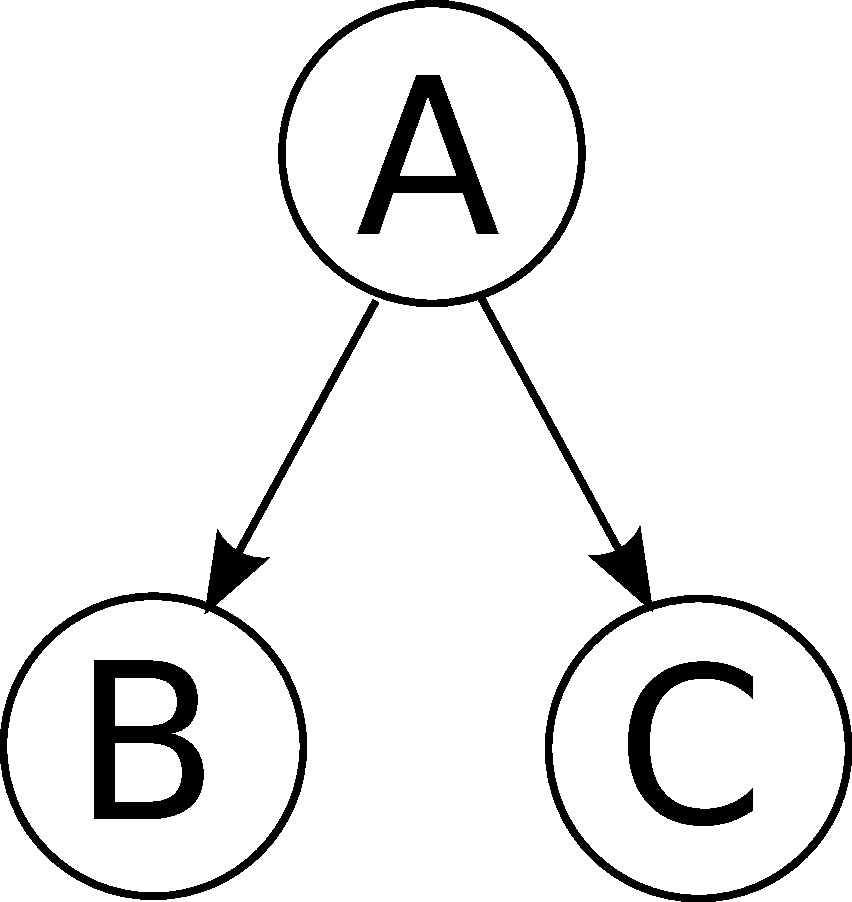
\includegraphics[height=0.2\textwidth]{Bayes1.pdf} \hspace{2em}
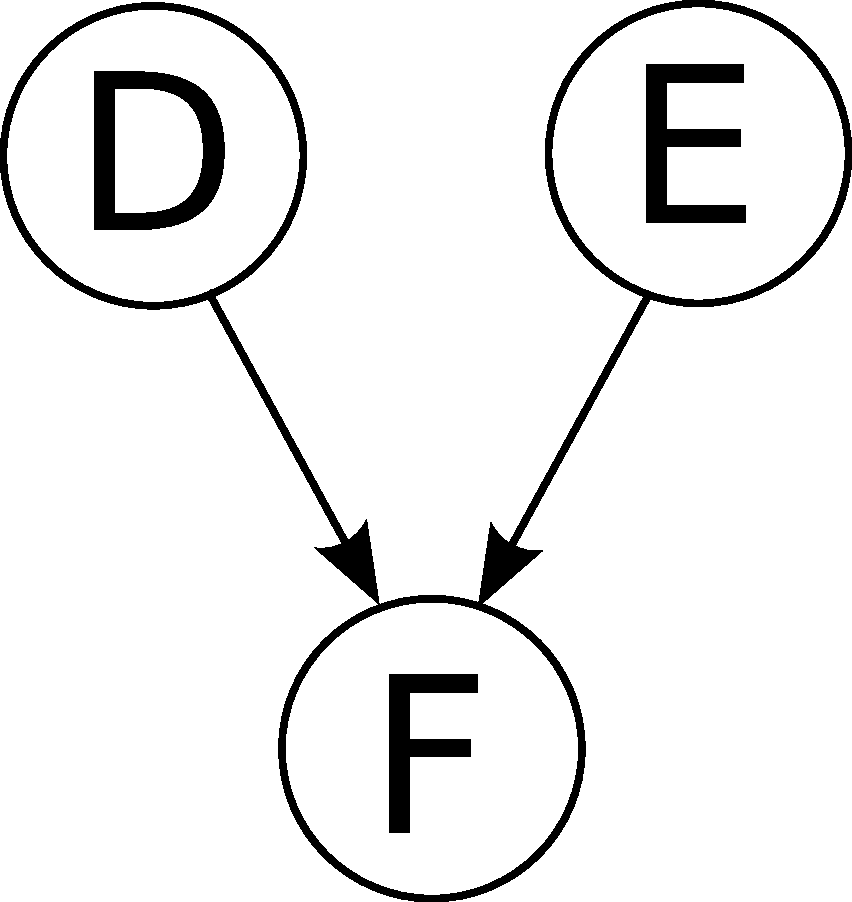
\includegraphics[height=0.2\textwidth]{Bayes2.pdf}
\end{figure}

To define the network on the left we need three values of probabilities: $P(A)$, $P(B|A)$ and $P(C|A)$. The probabilities of different values of events B and C depend on the value of the value of the event A. Thus the events B and C are dependent on event A. The events B and C conditionally independent given the value of A. However, if the value of A is not known, the events B and C are dependent on each other.

To define the network on the right we need to know $P(D)$, $P(E)$ and $P(F|D,E)$.The probability of different values of the event F is dependent on the values of the events D and E. Thus the event F is conditionally dependent on the events D and E. The events D and E are independent on each other if we don't know the value of the event F, but they are conditionally dependent given the value the event F.

\newpage

\begin{figure}[h!]
\centering
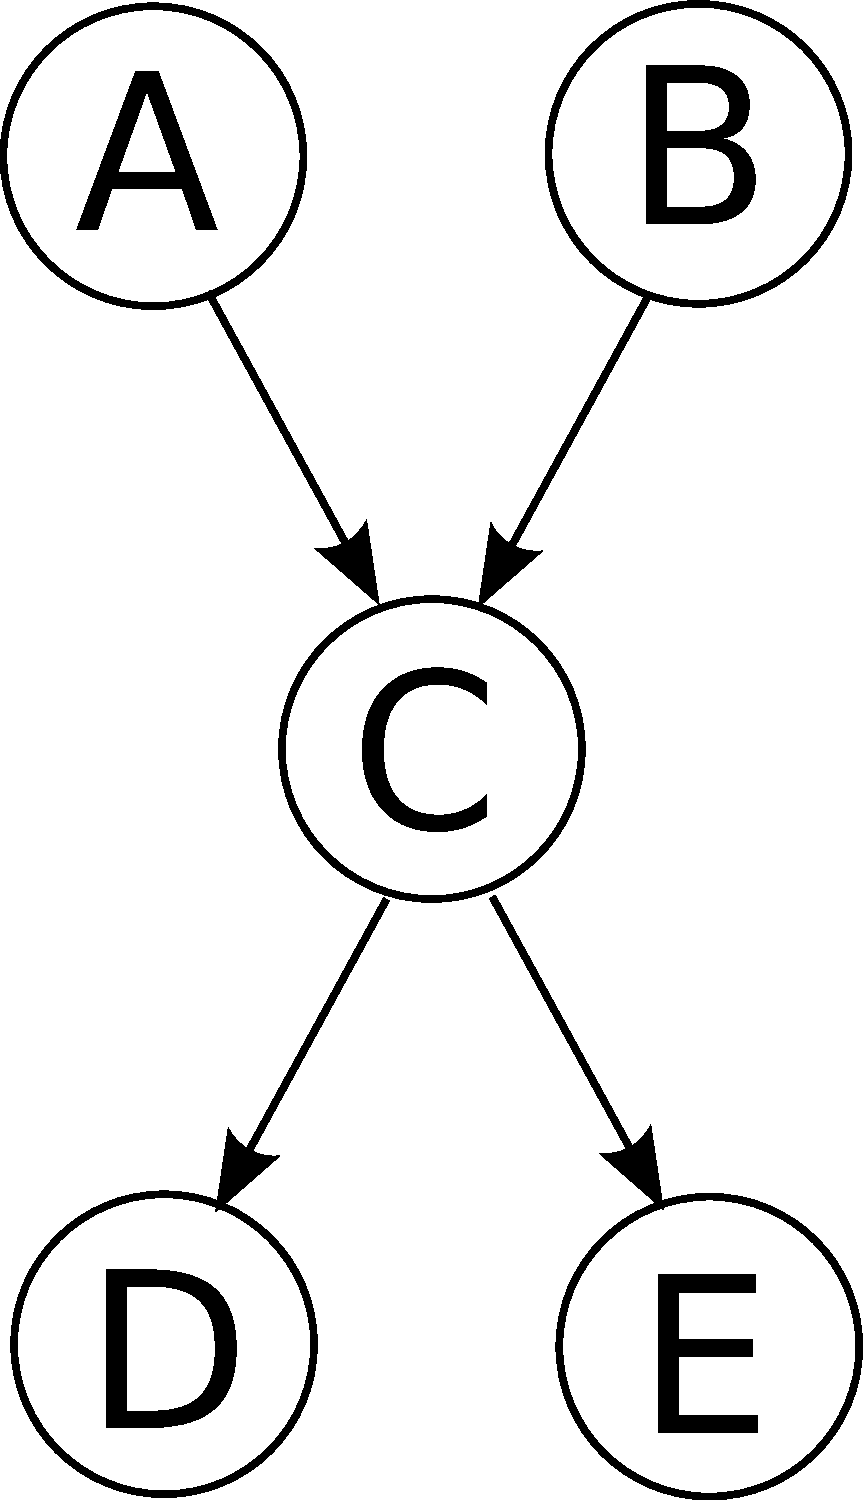
\includegraphics[height=0.3\textwidth]{Bayes3.pdf}
\end{figure}
To define such a distribution of probabilities we need to know $P(A)$ and $P(B)$, because they don't have the incoming edges, and the conditional distributions $P(C|A,B)$, $P(D|C)$ and $P(E|C)$. Thus we need 10 numerical values (in general $2^n$ values for each node with $n$ incoming edges). The joined distribution of all of the nodes in the network can be calculated as
\[ P(A,B,C,D,E) = P(A)P(B)P(C|A,B)P(D|C)P(E|C)\]


\end{document}